\subsection{Integration auf Datenebene}

für Data/Persistence Tier

\subsubsection{Gemeinsame Datenbank}

Zugriff meist über REST, GraphQL oder über das Extranet mit OData zwecks operativer aktueller Nutzung

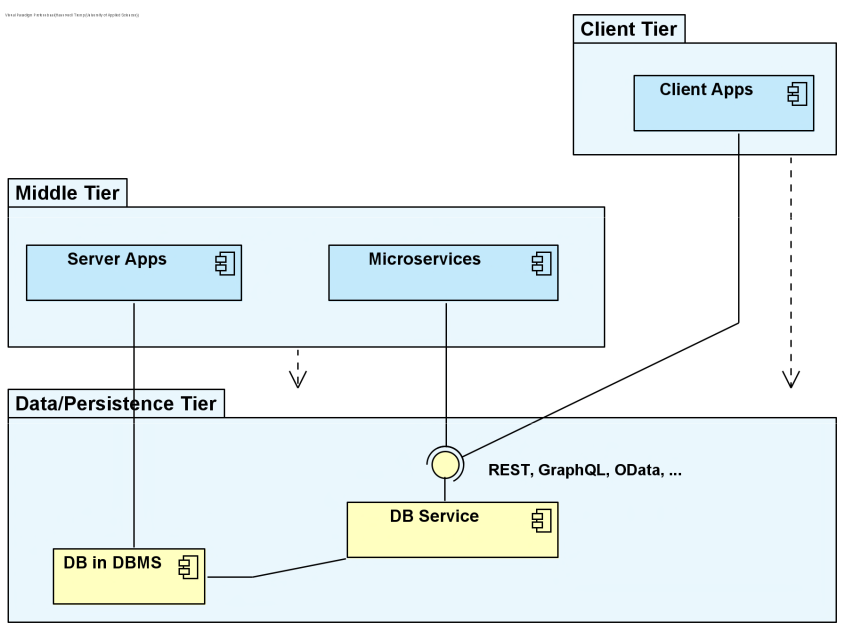
\includegraphics[width=\linewidth]{integration-datebase-shared.png}

\subsubsection{Zentrale, historisch orientierte Datenhaltung}

Zentrales Data Warehouse bzw. Data Lake zwecks Analyse

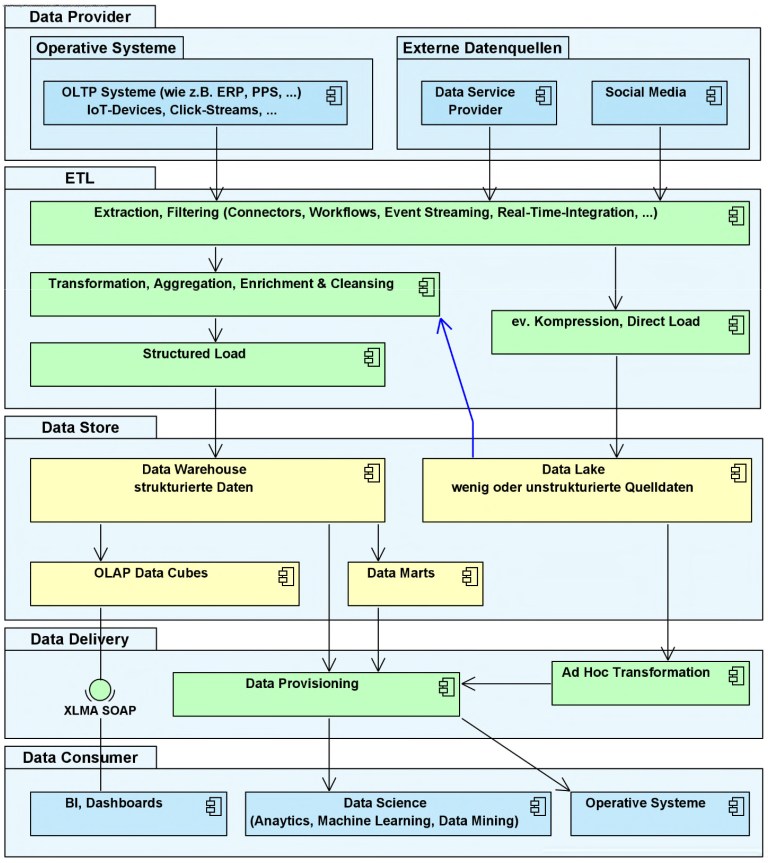
\includegraphics[width=\linewidth]{integration-datebase-central.png}

\begin{itemize}
    \item \textcolor{blue}{Data Warehouse} zentrales Datenmodell mit strukturierten Daten
    \item \textcolor{blue}{Data Lake} wenig / nicht strukturiert und meist 1:1 Quelldaten
    \item \textcolor{blue}{Data Marts} themenspezifische Auszüge aus Data Warehouse
\end{itemize}
\vspace{10pt}
\textbf{Aufbereitung der Daten für den Load}

\begin{itemize}
    \item \textcolor{blue}{Feldtransformation} Adressdaten sauber auseinander nehmen
    \item \textcolor{blue}{Codetransformation} einheitliche Codes im Data Warehouse
    \item \textcolor{blue}{Aggregation} nicht notwendige Detailtransaktionen
    \item \textcolor{blue}{Data-Enrichment} Adresse mit externen Marktinformationen anreichern
    \item \textcolor{blue}{Data-Cleansing} Daten überprüfen und bereinigen
\end{itemize}

\subsubsection{Prüfungsfragen}

\begin{itemize}
    \item Welches sind die in diesem Kapitel angesprochenen zwei Integrationsdimensionen? \\
    \textcolor{blue}{Organisationsinterne und organisationsübergreifende Integration}
    \item Auf welchen drei Ebenen kann die IT-Integration stattfinden? Auf welche Schichten
    des Mehrschichtenmodells beziehen sich diese? \\
    \textcolor{blue}{Präsentationsebene (Client Tier), Applikationsebene (Middle Tier) und Datenebene (Data / Persistence Tier)}
    \item Welche drei Varianten stehen bei der präsentationsorientierten
    Integration zur Verfügung? Nennen Sie zu jeder Variante je einen Vorteil \\
    \textcolor{blue}{Client-App-orientierte Integration, Portalorientierte Integration, Geschäftsprozessorientierte Integration}
    \item Welche wichtigen Funktionen übernimmt eine Integration Middleware (IM)? Geben Sie mindestens vier gebräuchliche synonyme Begriffe zu IM \\
    \textcolor{blue}{Integration Bus, Enterprise Service Bus, Integration Broker oder Hub}
    \item Zeichnen Sie mit dem UML-Komponentendiagramm gemäss den Vorgaben in diesem Kapitel die folgende Situation: ein ERP-System konsumiert den SOAP EDI-Service eines EDI-Service Providers und setzt dabei ebXML ein \\
    \textcolor{red}{Keine}
    \item Legen Sie den Unterschied zwischen einem Data Warehouse und einem Data Lake in 2-3 ganzen Sätzen dar \\
    \textcolor{blue}{Data Warehouse ist ein zentrales Datenmodell mit strukturierten Daten. Ein Data Lake hingegen hat wenig bis nicht strukturierte Daten, welche meist Quelldaten sind.}
    \item Über welche Schritte gelangen die Daten von einem ERP bis zu einer BI-Applikation? Geben Sie zu jedem Schritt eine kurze Erläuterung \\
    \textcolor{blue}{ETL (Extraction, Transformation, Load) $\rightarrow$ Data Store (Data Warehouse oder Data Lake) $\rightarrow$ BI Applikation}
\end{itemize}
